% ------------------------------------------------
% PHÂN TÍCH (Thành viên A). Ghép vào báo cáo chính bằng % ------------------------------------------------
% PHÂN TÍCH (Thành viên A). Ghép vào báo cáo chính bằng % ------------------------------------------------
% PHÂN TÍCH (Thành viên A). Ghép vào báo cáo chính bằng % ------------------------------------------------
% PHÂN TÍCH (Thành viên A). Ghép vào báo cáo chính bằng \input{analysis}
% Cần: booktabs, graphicx; hình trong figures/ (tạo bằng docs/report/make_figures.py)
% Số liệu: reports/errors/*_test, experiments/leakage, experiments/imbalance
% ------------------------------------------------

\section{Phân tích}
\label{sec:analysis}

Mục này dùng các mô hình cuối trên tập test (1.748 biển) để tách lỗi thành ba loại, theo cách ghép dự đoán với nhãn ở IoU $\geq 0{,}5$:
\begin{itemize}
\item \emph{bỏ sót}: không có dự đoán nào trùng biển;
\item \emph{nhầm lớp}: dự đoán trùng biển nhưng sai lớp;
\item \emph{báo nhầm nền}: dự đoán không trùng biển nào.
\end{itemize}
Ngưỡng độ tin cậy của mỗi mô hình được chọn sao cho F1 cao nhất, vì thang điểm tin cậy của YOLO và Faster R-CNN khác nhau. Phân tích trên tập val cho cùng các kết luận.

\subsection{Lỗi chính là bỏ sót biển nhỏ}
\label{sec:small}

Với YOLOv8s 1280, 77,1\% biển được tìm đúng, 21,1\% bị bỏ sót, và chỉ 1,9\% bị nhận sai lớp.
Trong 368 biển bị bỏ sót, 337 biển (92\%) nhỏ hơn 16 pixel. Hai mô hình còn lại cũng như vậy: 91\% với cắt ô + SAHI và 87\% với Faster R-CNN.
Hình~\ref{fig:recall-size} cho thấy với YOLO, recall gần như bão hòa ($> 92\%$) ở biển từ 16 pixel trở lên. Recall giảm ở biển 8--16 pixel, và ở biển dưới 8 pixel chỉ còn 21--39\% với cả ba mô hình.
Ở imgsz 1280, một biển 8 pixel trên ảnh gốc chỉ còn khoảng 6 pixel, nhỏ hơn một ô của bản đồ đặc trưng mịn nhất của YOLOv8 (stride 8). Cắt ô giữ nguyên độ phân giải gốc, nên tăng recall ở nhóm này từ 33,0\% lên 38,7\%.

Faster R-CNN kém YOLO ở mọi nhóm kích thước, kể cả nhóm $\geq 32$ pixel (93,6\% so với 96,4\%). Ảnh đưa vào Faster R-CNN còn lớn hơn (cạnh dài 1800 pixel), nên khoảng cách này không đến từ độ phân giải. Nhiều khả năng nó đến từ thiết lập huấn luyện: 30 epoch, augmentation đơn giản, so với 50 epoch có mosaic của YOLO. Faster R-CNN cũng báo nhầm nền nhiều hơn (156 so với 97 box).

\begin{figure}[t]
\centering
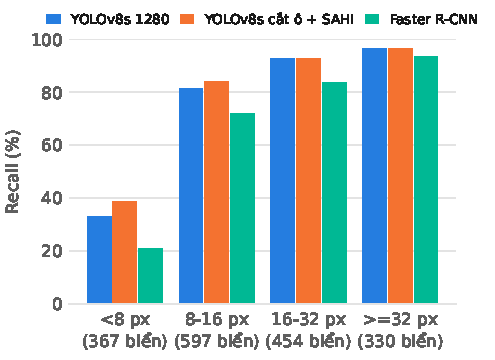
\includegraphics[width=\columnwidth]{figures/recall_theo_kich_thuoc.pdf}
\caption{Recall theo kích thước biển ($\sqrt{wh}$ trên ảnh gốc), tập test. Số dưới trục là số biển trong mỗi nhóm.}
\label{fig:recall-size}
\end{figure}

\subsection{Nhầm lớp tập trung ở ba lớp biển tròn viền đỏ}
\label{sec:confusion}

Ở YOLOv8s 1280, 30 trong 33 lần nhầm lớp (91\%) xảy ra giữa \textit{Cấm rẽ}, \textit{Giới hạn tốc độ} và \textit{Cấm còn lại}. Tỉ lệ bị gán sai lớp của ba lớp này lần lượt là 9,9\%, 11,4\% và 8,5\%, trong khi bốn lớp còn lại không quá 0,4\%.
Ba lớp này có cùng hình tròn, nền trắng, viền đỏ, chỉ khác hình vẽ ở giữa. Với biển 10 pixel, phần ở giữa chỉ còn vài pixel.
\textit{Cấm ngược chiều} là trường hợp ngược lại: lớp này có tới 90,5\% box nhỏ nhưng vẫn đạt AP50 84,7 trên test, vì nền đỏ đặc với vạch trắng ngang không giống lớp nào khác.
Vì vậy, độ khó của một lớp phụ thuộc vào việc nó có giống lớp khác không, hơn là vào kích thước biển.
Faster R-CNN nhầm nặng hơn hẳn: 28,4\% biển \textit{Cấm rẽ} bị gán sai lớp, chủ yếu thành \textit{Cấm còn lại}.

Nhóm xem lại bằng mắt cả 33 trường hợp nhầm lớp của YOLOv8s 1280:
\begin{itemize}
\item Ít nhất 7 trường hợp là \emph{nhãn sai, mô hình đúng}: biển ``50'' và ``80'' bị ghi \textit{Cấm còn lại}, biển hạn chế tải trọng ``10T'' bị ghi \textit{Giới hạn tốc độ}, biển tam giác cảnh báo bị ghi \textit{Hiệu lệnh}.
\item 4 trường hợp là lỗi rõ ràng của mô hình, ví dụ biển cấm rẽ rõ nét bị đoán thành \textit{Giới hạn tốc độ}.
\item Khoảng 19 trường hợp còn lại quá nhỏ hoặc quá mờ để người xem phân xử.
\end{itemize}

\subsection{Một phần ``báo nhầm nền'' là biển thiếu nhãn}
\label{sec:missing-labels}

Nhóm cũng xem lại 28 dự đoán bị tính là báo nhầm nền có độ tin cậy $\geq 0{,}6$, tức là các dự đoán không chồng lên box thật nào.
Ít nhất 15 trường hợp trúng một biển báo rõ ràng thuộc 7 lớp nhưng không được gán nhãn. Ví dụ: biển cấm đỗ và biển cấm rẽ trên cùng một cột, biển cảnh báo tam giác, biển ``10'' (Hình~\ref{fig:examples}, cột cuối).
Khoảng 5 trường hợp khác có thể cũng là biển. Chỉ khoảng 8 trường hợp là nền thật, chủ yếu là các mảng tối mờ.
Như vậy, nhãn test vừa thiếu biển vừa có nhãn sai lớp, và cả hai đều làm điểm của mô hình thấp hơn khả năng thật. Mức chênh này chưa được định lượng.

\begin{figure*}[t]
\centering
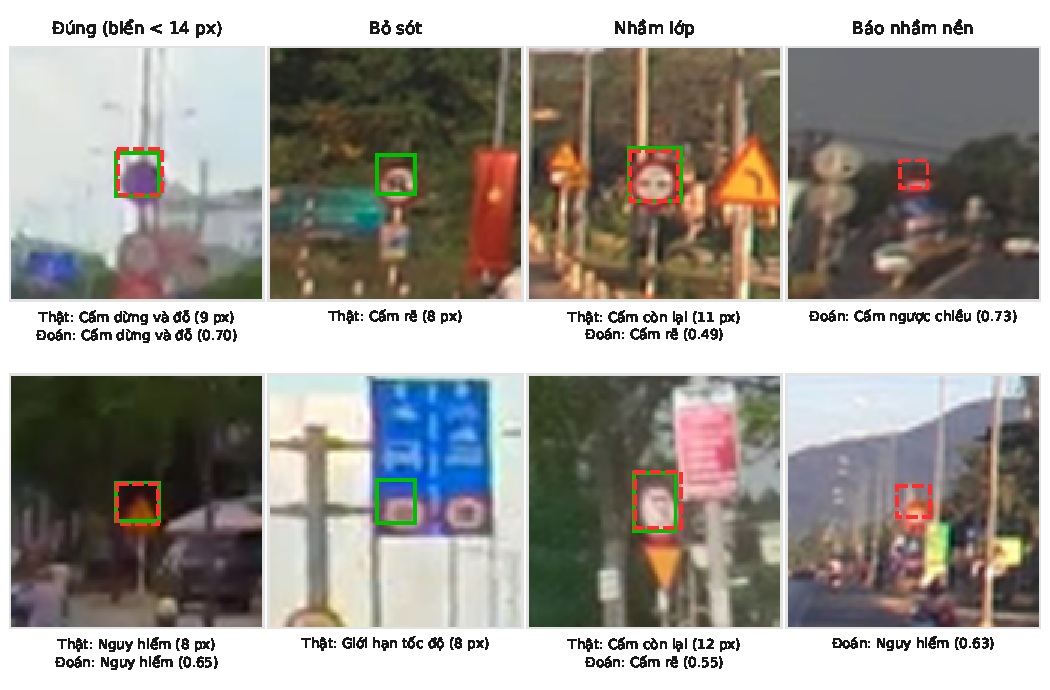
\includegraphics[width=0.92\textwidth]{figures/vi_du_du_doan.pdf}
\caption{Ví dụ dự đoán của YOLOv8s 1280 trên tập test (khung xanh liền: nhãn thật; khung đỏ đứt: dự đoán).
Cột 3, hàng dưới: biển có mũi tên rẽ bị gạch (\textit{Cấm rẽ}) nhưng bị gán nhãn \textit{Cấm còn lại}, nên dự đoán đúng của mô hình bị tính là nhầm lớp.
Cột 4: dự đoán không có nhãn thật tương ứng; hàng dưới trúng một biển thật không được gán nhãn.}
\label{fig:examples}
\end{figure*}

\subsection{Biển đứng cụm không bị bỏ sót nhiều hơn}
\label{sec:clusters}

43\% biển trong test đứng sát một biển khác (khe hở nhỏ hơn nửa cạnh của biển nhỏ hơn), thường là nhiều biển gắn trên cùng một cột.
Nếu chỉ nhìn số chung, biển trong cụm có vẻ bị bỏ sót nhiều hơn: recall 73,8\% so với 79,5\% với YOLOv8s 1280.
Nhưng biển trong cụm nhỏ hơn nhiều: 67,6\% dưới 16 pixel, so với 45,8\% ở biển đứng riêng.
Khi so trong từng nhóm kích thước, biển trong cụm được tìm thấy ngang bằng hoặc nhiều hơn (8--16 pixel: 86,0\% so với 77,7\%).
Vậy chênh lệch chung là do kích thước biển (biến gây nhiễu), không phải do NMS xóa nhầm biển đứng sát nhau. Ngưỡng NMS 0,65 theo từng lớp là đủ an toàn.

\subsection{Thí nghiệm: rò rỉ dữ liệu khi chia ngẫu nhiên}
\label{sec:leakage}

Để đo tác động của cách chia tập, nhóm lấy tập train (2.933 ảnh, 28 tuyến đường) chia lại thành train$'$/val$'$ (1.994/939 ảnh) theo hai cách: ngẫu nhiên theo ảnh, và theo tuyến đường.
Hai mô hình YOLOv8n (imgsz 1280, 50 epoch, cùng seed) được huấn luyện giống hệt nhau, chỉ khác cách chia.
Cả hai được chấm trên val$'$ của chính nó, và trên tập val gốc gồm 5 tuyến đường cả hai chưa từng thấy (Bảng~\ref{tab:leakage}). Tập test không được dùng trong thí nghiệm này.

\begin{table}[t]
\centering
\small
\begin{tabular}{lccc}
\toprule
Cách chia & val$'$ & Đường mới & Chênh \\
\midrule
Ngẫu nhiên    & \textbf{78,5} & \textbf{72,8} & $+5{,}7$ \\
Theo đường    & 62,9 & 69,9 & $-7{,}0$ \\
\bottomrule
\end{tabular}
\caption{mAP@0.5 (\%) của thí nghiệm rò rỉ. Với cách chia ngẫu nhiên, 88\% ảnh val$'$ có khung hình liền kề nằm trong train$'$.}
\label{tab:leakage}
\end{table}

Trên val$'$, mô hình chia ngẫu nhiên hơn mô hình chia theo đường 15,6 điểm. Trên cùng các tuyến đường mới, nó chỉ hơn 2,9 điểm.
Vậy phần lớn khoảng cách trên val$'$ là ảo: 88\% ảnh val$'$ có một khung hình gần như giống hệt trong train$'$.
Nếu tin vào val$'$ chia ngẫu nhiên, ta đánh giá khả năng trên đường mới cao hơn thực tế 5,7 điểm.
Phần hơn 2,9 điểm còn lại có thể vì mô hình chia ngẫu nhiên được thấy cả 28 tuyến đường, còn mô hình kia chỉ thấy 23.
Thí nghiệm cũng cho thấy hai bộ 5 tuyến đường có thể chênh nhau tới 7 điểm (62,9 so với 69,9). Điều này giúp giải thích vì sao kết quả trên val và test của nhóm lệch nhau 5--6 điểm.

\subsection{Thí nghiệm: xử lý mất cân bằng lớp}
\label{sec:imbalance}

Mục~\ref{sec:confusion} cho thấy các lớp ít mẫu (\textit{Cấm rẽ}, \textit{Giới hạn tốc độ}) cũng là các lớp hay bị nhầm. Nhóm thử hai cách cân bằng lớp trên cấu hình YOLOv8s 1280, mỗi cách chỉ thay đổi đúng một yếu tố:
\begin{itemize}
\item \textbf{Repeat Factor Sampling} (RFS) \citep{gupta2019lvis}: lặp lại các ảnh chứa lớp hiếm với hệ số $r_c = \max(1, \sqrt{t/f_c})$, trong đó $f_c$ là tỉ lệ ảnh có lớp $c$ và $t = 0{,}3$. Cách này giảm tỉ lệ số box lớp nhiều nhất / ít nhất từ 4,4 xuống 2,9.
\item \textbf{Trọng số lớp} trong loss phân loại, tỉ lệ với $(1/n_c)^{0{,}5}$, trong đó $n_c$ là số box của lớp $c$ (tham số \texttt{cls\_pw} của Ultralytics).
\end{itemize}

\begin{table}[t]
\centering
\small
\begin{tabular}{lccc}
\toprule
& Gốc & RFS & Trọng số lớp \\
\midrule
mAP@0.5          & \textbf{82,2} & 81,0 & 81,1 \\
AP50 Cấm rẽ          & \textbf{75,0} & 71,4 & 74,9 \\
AP50 Giới hạn tốc độ & \textbf{77,7} & 73,1 & 71,6$^{*}$ \\
AP50 Hiệu lệnh       & 78,6 & \textbf{80,7} & 78,7 \\
Nhầm trong nhóm tròn đỏ & \textbf{47} & 56 & 50 \\
\bottomrule
\end{tabular}
\caption{Thí nghiệm mất cân bằng lớp trên val (\%). Dòng cuối là số biển bị nhầm giữa ba lớp tròn viền đỏ. $^{*}$: chênh lệch so với gốc có ý nghĩa thống kê (bootstrap, khoảng tin cậy 95\% là $[-10{,}2; -1{,}6]$). Mọi chênh lệch khác đều nằm trong khoảng dao động.}
\label{tab:imbalance}
\end{table}

Cả hai cách đều \emph{không} cải thiện các lớp hiếm (Bảng~\ref{tab:imbalance}). Có bốn nguyên nhân:
\begin{enumerate}
\item \textbf{Lỗi chỉ bị chuyển chỗ, không mất đi.} Tổng số lần nhầm trong nhóm tròn đỏ không giảm (47 tăng lên 56 và 50).
  Với trọng số lớp, \textit{Cấm rẽ} được nhận đúng thêm 3 biển, nhưng số dự đoán \textit{Cấm rẽ} sai tăng từ 9 lên 17. \textit{Giới hạn tốc độ} bị kéo sang \textit{Cấm rẽ} nhiều hơn, nên AP của nó giảm 6,1 điểm.
  Trọng số chỉ dịch ranh giới quyết định giữa các lớp trông giống nhau, chứ không giúp phân biệt chúng tốt hơn.
\item \textbf{Lặp ảnh thì lặp luôn lớp gây nhầm.} 49\% ảnh có \textit{Giới hạn tốc độ} cũng có \textit{Cấm còn lại}, trong khi tỉ lệ chung chỉ 25\%. Vì vậy RFS lặp chính lớp mà \textit{Giới hạn tốc độ} hay bị nhầm sang.
\item \textbf{Nhầm lớp không phải lỗi chính.} Chỉ 3,2\% biển bị nhầm lớp, trong khi 16,7\% bị bỏ sót (Mục~\ref{sec:small}). Cân bằng lớp không làm recall biển nhỏ tăng.
\item \textbf{Mức mất cân bằng vừa phải} (4,4 lần). RFS được thiết kế cho dữ liệu đuôi dài, nơi lớp hiếm ít hơn hàng trăm lần.
\end{enumerate}
Không thấy dấu hiệu học thuộc do lặp ảnh: loss phân loại trên val vẫn giảm tới epoch cuối.
Với nhầm lẫn giữa các lớp tròn viền đỏ, cách hợp lý hơn là cho mô hình nhìn rõ phần giữa biển (độ phân giải cao hơn, hoặc phân loại lại vùng cắt quanh biển) và sửa nhãn sai (Mục~\ref{sec:confusion}).

\subsection{Hạn chế}
\label{sec:limitations}

\begin{itemize}
\item \textbf{Nhãn còn nhiễu.} Box trùng đã được gộp, nhưng nhãn sai lớp và biển thiếu nhãn vẫn còn (Mục~\ref{sec:confusion} và \ref{sec:missing-labels}). Điểm trên test vì vậy là cận dưới của khả năng thật.
\item \textbf{Ít tuyến đường.} Val và test mỗi tập chỉ có 5 tuyến đường. Kết quả có thể lệch vài điểm tùy tuyến đường nào rơi vào tập nào (Mục~\ref{sec:leakage}).
\item \textbf{Mỗi cấu hình chỉ huấn luyện một lần.} Khoảng tin cậy bootstrap chỉ tính dao động do chọn ảnh, chưa tính dao động giữa các lần huấn luyện.
\item \textbf{AP\textsubscript{L} không đáng tin.} Val chỉ có 23 biển lớn và test có 34, nên nhóm không so sánh AP\textsubscript{L}.
\item \textbf{Ngưỡng xuất dự đoán của Faster R-CNN trên val} là 0,05 thay vì 0,001, nên mAP trên val của Faster R-CNN có thể thấp hơn thực tế một chút. Trên test thì không có vấn đề này.
\end{itemize}

% Cần: booktabs, graphicx; hình trong figures/ (tạo bằng docs/report/make_figures.py)
% Số liệu: reports/errors/*_test, experiments/leakage, experiments/imbalance
% ------------------------------------------------

\section{Phân tích}
\label{sec:analysis}

Mục này dùng các mô hình cuối trên tập test (1.748 biển) để tách lỗi thành ba loại, theo cách ghép dự đoán với nhãn ở IoU $\geq 0{,}5$:
\begin{itemize}
\item \emph{bỏ sót}: không có dự đoán nào trùng biển;
\item \emph{nhầm lớp}: dự đoán trùng biển nhưng sai lớp;
\item \emph{báo nhầm nền}: dự đoán không trùng biển nào.
\end{itemize}
Ngưỡng độ tin cậy của mỗi mô hình được chọn sao cho F1 cao nhất, vì thang điểm tin cậy của YOLO và Faster R-CNN khác nhau. Phân tích trên tập val cho cùng các kết luận.

\subsection{Lỗi chính là bỏ sót biển nhỏ}
\label{sec:small}

Với YOLOv8s 1280, 77,1\% biển được tìm đúng, 21,1\% bị bỏ sót, và chỉ 1,9\% bị nhận sai lớp.
Trong 368 biển bị bỏ sót, 337 biển (92\%) nhỏ hơn 16 pixel. Hai mô hình còn lại cũng như vậy: 91\% với cắt ô + SAHI và 87\% với Faster R-CNN.
Hình~\ref{fig:recall-size} cho thấy với YOLO, recall gần như bão hòa ($> 92\%$) ở biển từ 16 pixel trở lên. Recall giảm ở biển 8--16 pixel, và ở biển dưới 8 pixel chỉ còn 21--39\% với cả ba mô hình.
Ở imgsz 1280, một biển 8 pixel trên ảnh gốc chỉ còn khoảng 6 pixel, nhỏ hơn một ô của bản đồ đặc trưng mịn nhất của YOLOv8 (stride 8). Cắt ô giữ nguyên độ phân giải gốc, nên tăng recall ở nhóm này từ 33,0\% lên 38,7\%.

Faster R-CNN kém YOLO ở mọi nhóm kích thước, kể cả nhóm $\geq 32$ pixel (93,6\% so với 96,4\%). Ảnh đưa vào Faster R-CNN còn lớn hơn (cạnh dài 1800 pixel), nên khoảng cách này không đến từ độ phân giải. Nhiều khả năng nó đến từ thiết lập huấn luyện: 30 epoch, augmentation đơn giản, so với 50 epoch có mosaic của YOLO. Faster R-CNN cũng báo nhầm nền nhiều hơn (156 so với 97 box).

\begin{figure}[t]
\centering
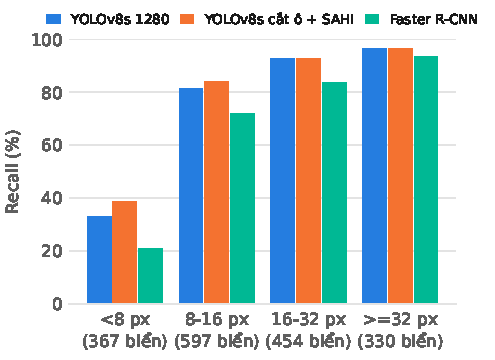
\includegraphics[width=\columnwidth]{figures/recall_theo_kich_thuoc.pdf}
\caption{Recall theo kích thước biển ($\sqrt{wh}$ trên ảnh gốc), tập test. Số dưới trục là số biển trong mỗi nhóm.}
\label{fig:recall-size}
\end{figure}

\subsection{Nhầm lớp tập trung ở ba lớp biển tròn viền đỏ}
\label{sec:confusion}

Ở YOLOv8s 1280, 30 trong 33 lần nhầm lớp (91\%) xảy ra giữa \textit{Cấm rẽ}, \textit{Giới hạn tốc độ} và \textit{Cấm còn lại}. Tỉ lệ bị gán sai lớp của ba lớp này lần lượt là 9,9\%, 11,4\% và 8,5\%, trong khi bốn lớp còn lại không quá 0,4\%.
Ba lớp này có cùng hình tròn, nền trắng, viền đỏ, chỉ khác hình vẽ ở giữa. Với biển 10 pixel, phần ở giữa chỉ còn vài pixel.
\textit{Cấm ngược chiều} là trường hợp ngược lại: lớp này có tới 90,5\% box nhỏ nhưng vẫn đạt AP50 84,7 trên test, vì nền đỏ đặc với vạch trắng ngang không giống lớp nào khác.
Vì vậy, độ khó của một lớp phụ thuộc vào việc nó có giống lớp khác không, hơn là vào kích thước biển.
Faster R-CNN nhầm nặng hơn hẳn: 28,4\% biển \textit{Cấm rẽ} bị gán sai lớp, chủ yếu thành \textit{Cấm còn lại}.

Nhóm xem lại bằng mắt cả 33 trường hợp nhầm lớp của YOLOv8s 1280:
\begin{itemize}
\item Ít nhất 7 trường hợp là \emph{nhãn sai, mô hình đúng}: biển ``50'' và ``80'' bị ghi \textit{Cấm còn lại}, biển hạn chế tải trọng ``10T'' bị ghi \textit{Giới hạn tốc độ}, biển tam giác cảnh báo bị ghi \textit{Hiệu lệnh}.
\item 4 trường hợp là lỗi rõ ràng của mô hình, ví dụ biển cấm rẽ rõ nét bị đoán thành \textit{Giới hạn tốc độ}.
\item Khoảng 19 trường hợp còn lại quá nhỏ hoặc quá mờ để người xem phân xử.
\end{itemize}

\subsection{Một phần ``báo nhầm nền'' là biển thiếu nhãn}
\label{sec:missing-labels}

Nhóm cũng xem lại 28 dự đoán bị tính là báo nhầm nền có độ tin cậy $\geq 0{,}6$, tức là các dự đoán không chồng lên box thật nào.
Ít nhất 15 trường hợp trúng một biển báo rõ ràng thuộc 7 lớp nhưng không được gán nhãn. Ví dụ: biển cấm đỗ và biển cấm rẽ trên cùng một cột, biển cảnh báo tam giác, biển ``10'' (Hình~\ref{fig:examples}, cột cuối).
Khoảng 5 trường hợp khác có thể cũng là biển. Chỉ khoảng 8 trường hợp là nền thật, chủ yếu là các mảng tối mờ.
Như vậy, nhãn test vừa thiếu biển vừa có nhãn sai lớp, và cả hai đều làm điểm của mô hình thấp hơn khả năng thật. Mức chênh này chưa được định lượng.

\begin{figure*}[t]
\centering
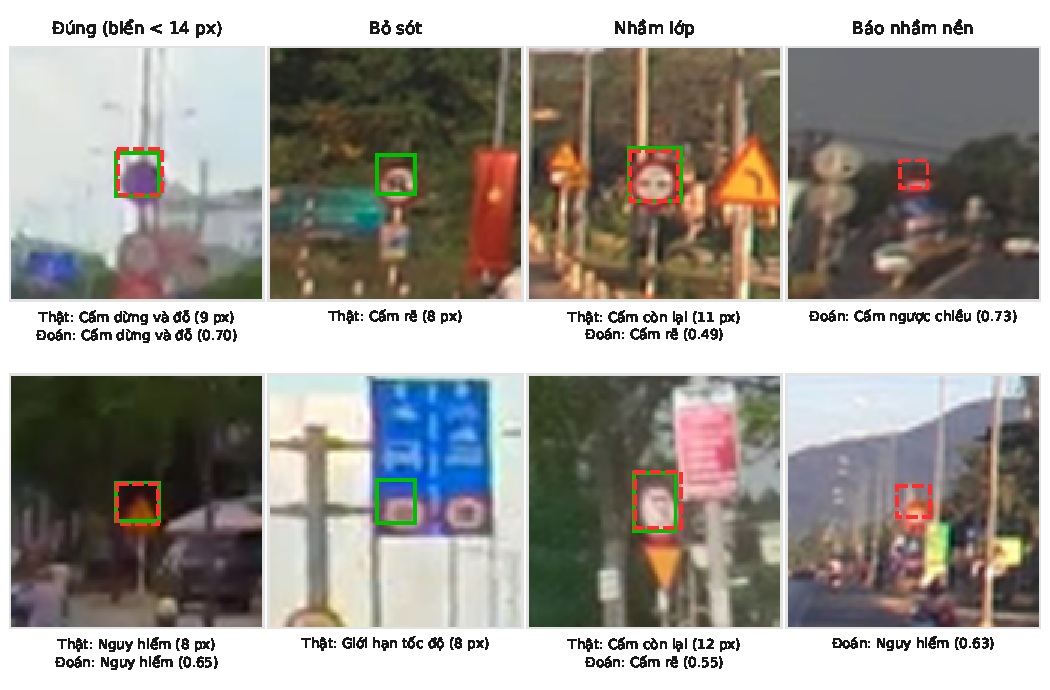
\includegraphics[width=0.92\textwidth]{figures/vi_du_du_doan.pdf}
\caption{Ví dụ dự đoán của YOLOv8s 1280 trên tập test (khung xanh liền: nhãn thật; khung đỏ đứt: dự đoán).
Cột 3, hàng dưới: biển có mũi tên rẽ bị gạch (\textit{Cấm rẽ}) nhưng bị gán nhãn \textit{Cấm còn lại}, nên dự đoán đúng của mô hình bị tính là nhầm lớp.
Cột 4: dự đoán không có nhãn thật tương ứng; hàng dưới trúng một biển thật không được gán nhãn.}
\label{fig:examples}
\end{figure*}

\subsection{Biển đứng cụm không bị bỏ sót nhiều hơn}
\label{sec:clusters}

43\% biển trong test đứng sát một biển khác (khe hở nhỏ hơn nửa cạnh của biển nhỏ hơn), thường là nhiều biển gắn trên cùng một cột.
Nếu chỉ nhìn số chung, biển trong cụm có vẻ bị bỏ sót nhiều hơn: recall 73,8\% so với 79,5\% với YOLOv8s 1280.
Nhưng biển trong cụm nhỏ hơn nhiều: 67,6\% dưới 16 pixel, so với 45,8\% ở biển đứng riêng.
Khi so trong từng nhóm kích thước, biển trong cụm được tìm thấy ngang bằng hoặc nhiều hơn (8--16 pixel: 86,0\% so với 77,7\%).
Vậy chênh lệch chung là do kích thước biển (biến gây nhiễu), không phải do NMS xóa nhầm biển đứng sát nhau. Ngưỡng NMS 0,65 theo từng lớp là đủ an toàn.

\subsection{Thí nghiệm: rò rỉ dữ liệu khi chia ngẫu nhiên}
\label{sec:leakage}

Để đo tác động của cách chia tập, nhóm lấy tập train (2.933 ảnh, 28 tuyến đường) chia lại thành train$'$/val$'$ (1.994/939 ảnh) theo hai cách: ngẫu nhiên theo ảnh, và theo tuyến đường.
Hai mô hình YOLOv8n (imgsz 1280, 50 epoch, cùng seed) được huấn luyện giống hệt nhau, chỉ khác cách chia.
Cả hai được chấm trên val$'$ của chính nó, và trên tập val gốc gồm 5 tuyến đường cả hai chưa từng thấy (Bảng~\ref{tab:leakage}). Tập test không được dùng trong thí nghiệm này.

\begin{table}[t]
\centering
\small
\begin{tabular}{lccc}
\toprule
Cách chia & val$'$ & Đường mới & Chênh \\
\midrule
Ngẫu nhiên    & \textbf{78,5} & \textbf{72,8} & $+5{,}7$ \\
Theo đường    & 62,9 & 69,9 & $-7{,}0$ \\
\bottomrule
\end{tabular}
\caption{mAP@0.5 (\%) của thí nghiệm rò rỉ. Với cách chia ngẫu nhiên, 88\% ảnh val$'$ có khung hình liền kề nằm trong train$'$.}
\label{tab:leakage}
\end{table}

Trên val$'$, mô hình chia ngẫu nhiên hơn mô hình chia theo đường 15,6 điểm. Trên cùng các tuyến đường mới, nó chỉ hơn 2,9 điểm.
Vậy phần lớn khoảng cách trên val$'$ là ảo: 88\% ảnh val$'$ có một khung hình gần như giống hệt trong train$'$.
Nếu tin vào val$'$ chia ngẫu nhiên, ta đánh giá khả năng trên đường mới cao hơn thực tế 5,7 điểm.
Phần hơn 2,9 điểm còn lại có thể vì mô hình chia ngẫu nhiên được thấy cả 28 tuyến đường, còn mô hình kia chỉ thấy 23.
Thí nghiệm cũng cho thấy hai bộ 5 tuyến đường có thể chênh nhau tới 7 điểm (62,9 so với 69,9). Điều này giúp giải thích vì sao kết quả trên val và test của nhóm lệch nhau 5--6 điểm.

\subsection{Thí nghiệm: xử lý mất cân bằng lớp}
\label{sec:imbalance}

Mục~\ref{sec:confusion} cho thấy các lớp ít mẫu (\textit{Cấm rẽ}, \textit{Giới hạn tốc độ}) cũng là các lớp hay bị nhầm. Nhóm thử hai cách cân bằng lớp trên cấu hình YOLOv8s 1280, mỗi cách chỉ thay đổi đúng một yếu tố:
\begin{itemize}
\item \textbf{Repeat Factor Sampling} (RFS) \citep{gupta2019lvis}: lặp lại các ảnh chứa lớp hiếm với hệ số $r_c = \max(1, \sqrt{t/f_c})$, trong đó $f_c$ là tỉ lệ ảnh có lớp $c$ và $t = 0{,}3$. Cách này giảm tỉ lệ số box lớp nhiều nhất / ít nhất từ 4,4 xuống 2,9.
\item \textbf{Trọng số lớp} trong loss phân loại, tỉ lệ với $(1/n_c)^{0{,}5}$, trong đó $n_c$ là số box của lớp $c$ (tham số \texttt{cls\_pw} của Ultralytics).
\end{itemize}

\begin{table}[t]
\centering
\small
\begin{tabular}{lccc}
\toprule
& Gốc & RFS & Trọng số lớp \\
\midrule
mAP@0.5          & \textbf{82,2} & 81,0 & 81,1 \\
AP50 Cấm rẽ          & \textbf{75,0} & 71,4 & 74,9 \\
AP50 Giới hạn tốc độ & \textbf{77,7} & 73,1 & 71,6$^{*}$ \\
AP50 Hiệu lệnh       & 78,6 & \textbf{80,7} & 78,7 \\
Nhầm trong nhóm tròn đỏ & \textbf{47} & 56 & 50 \\
\bottomrule
\end{tabular}
\caption{Thí nghiệm mất cân bằng lớp trên val (\%). Dòng cuối là số biển bị nhầm giữa ba lớp tròn viền đỏ. $^{*}$: chênh lệch so với gốc có ý nghĩa thống kê (bootstrap, khoảng tin cậy 95\% là $[-10{,}2; -1{,}6]$). Mọi chênh lệch khác đều nằm trong khoảng dao động.}
\label{tab:imbalance}
\end{table}

Cả hai cách đều \emph{không} cải thiện các lớp hiếm (Bảng~\ref{tab:imbalance}). Có bốn nguyên nhân:
\begin{enumerate}
\item \textbf{Lỗi chỉ bị chuyển chỗ, không mất đi.} Tổng số lần nhầm trong nhóm tròn đỏ không giảm (47 tăng lên 56 và 50).
  Với trọng số lớp, \textit{Cấm rẽ} được nhận đúng thêm 3 biển, nhưng số dự đoán \textit{Cấm rẽ} sai tăng từ 9 lên 17. \textit{Giới hạn tốc độ} bị kéo sang \textit{Cấm rẽ} nhiều hơn, nên AP của nó giảm 6,1 điểm.
  Trọng số chỉ dịch ranh giới quyết định giữa các lớp trông giống nhau, chứ không giúp phân biệt chúng tốt hơn.
\item \textbf{Lặp ảnh thì lặp luôn lớp gây nhầm.} 49\% ảnh có \textit{Giới hạn tốc độ} cũng có \textit{Cấm còn lại}, trong khi tỉ lệ chung chỉ 25\%. Vì vậy RFS lặp chính lớp mà \textit{Giới hạn tốc độ} hay bị nhầm sang.
\item \textbf{Nhầm lớp không phải lỗi chính.} Chỉ 3,2\% biển bị nhầm lớp, trong khi 16,7\% bị bỏ sót (Mục~\ref{sec:small}). Cân bằng lớp không làm recall biển nhỏ tăng.
\item \textbf{Mức mất cân bằng vừa phải} (4,4 lần). RFS được thiết kế cho dữ liệu đuôi dài, nơi lớp hiếm ít hơn hàng trăm lần.
\end{enumerate}
Không thấy dấu hiệu học thuộc do lặp ảnh: loss phân loại trên val vẫn giảm tới epoch cuối.
Với nhầm lẫn giữa các lớp tròn viền đỏ, cách hợp lý hơn là cho mô hình nhìn rõ phần giữa biển (độ phân giải cao hơn, hoặc phân loại lại vùng cắt quanh biển) và sửa nhãn sai (Mục~\ref{sec:confusion}).

\subsection{Hạn chế}
\label{sec:limitations}

\begin{itemize}
\item \textbf{Nhãn còn nhiễu.} Box trùng đã được gộp, nhưng nhãn sai lớp và biển thiếu nhãn vẫn còn (Mục~\ref{sec:confusion} và \ref{sec:missing-labels}). Điểm trên test vì vậy là cận dưới của khả năng thật.
\item \textbf{Ít tuyến đường.} Val và test mỗi tập chỉ có 5 tuyến đường. Kết quả có thể lệch vài điểm tùy tuyến đường nào rơi vào tập nào (Mục~\ref{sec:leakage}).
\item \textbf{Mỗi cấu hình chỉ huấn luyện một lần.} Khoảng tin cậy bootstrap chỉ tính dao động do chọn ảnh, chưa tính dao động giữa các lần huấn luyện.
\item \textbf{AP\textsubscript{L} không đáng tin.} Val chỉ có 23 biển lớn và test có 34, nên nhóm không so sánh AP\textsubscript{L}.
\item \textbf{Ngưỡng xuất dự đoán của Faster R-CNN trên val} là 0,05 thay vì 0,001, nên mAP trên val của Faster R-CNN có thể thấp hơn thực tế một chút. Trên test thì không có vấn đề này.
\end{itemize}

% Cần: booktabs, graphicx; hình trong figures/ (tạo bằng docs/report/make_figures.py)
% Số liệu: reports/errors/*_test, experiments/leakage, experiments/imbalance
% ------------------------------------------------

\section{Phân tích}
\label{sec:analysis}

Mục này dùng các mô hình cuối trên tập test (1.748 biển) để tách lỗi thành ba loại, theo cách ghép dự đoán với nhãn ở IoU $\geq 0{,}5$:
\begin{itemize}
\item \emph{bỏ sót}: không có dự đoán nào trùng biển;
\item \emph{nhầm lớp}: dự đoán trùng biển nhưng sai lớp;
\item \emph{báo nhầm nền}: dự đoán không trùng biển nào.
\end{itemize}
Ngưỡng độ tin cậy của mỗi mô hình được chọn sao cho F1 cao nhất, vì thang điểm tin cậy của YOLO và Faster R-CNN khác nhau. Phân tích trên tập val cho cùng các kết luận.

\subsection{Lỗi chính là bỏ sót biển nhỏ}
\label{sec:small}

Với YOLOv8s 1280, 77,1\% biển được tìm đúng, 21,1\% bị bỏ sót, và chỉ 1,9\% bị nhận sai lớp.
Trong 368 biển bị bỏ sót, 337 biển (92\%) nhỏ hơn 16 pixel. Hai mô hình còn lại cũng như vậy: 91\% với cắt ô + SAHI và 87\% với Faster R-CNN.
Hình~\ref{fig:recall-size} cho thấy với YOLO, recall gần như bão hòa ($> 92\%$) ở biển từ 16 pixel trở lên. Recall giảm ở biển 8--16 pixel, và ở biển dưới 8 pixel chỉ còn 21--39\% với cả ba mô hình.
Ở imgsz 1280, một biển 8 pixel trên ảnh gốc chỉ còn khoảng 6 pixel, nhỏ hơn một ô của bản đồ đặc trưng mịn nhất của YOLOv8 (stride 8). Cắt ô giữ nguyên độ phân giải gốc, nên tăng recall ở nhóm này từ 33,0\% lên 38,7\%.

Faster R-CNN kém YOLO ở mọi nhóm kích thước, kể cả nhóm $\geq 32$ pixel (93,6\% so với 96,4\%). Ảnh đưa vào Faster R-CNN còn lớn hơn (cạnh dài 1800 pixel), nên khoảng cách này không đến từ độ phân giải. Nhiều khả năng nó đến từ thiết lập huấn luyện: 30 epoch, augmentation đơn giản, so với 50 epoch có mosaic của YOLO. Faster R-CNN cũng báo nhầm nền nhiều hơn (156 so với 97 box).

\begin{figure}[t]
\centering
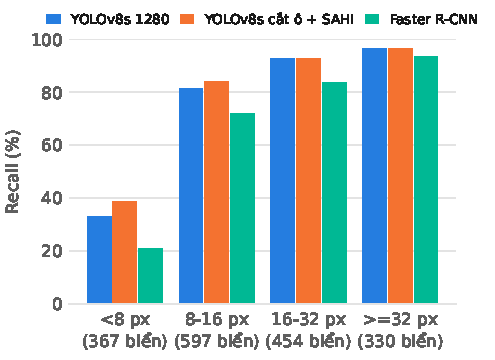
\includegraphics[width=\columnwidth]{figures/recall_theo_kich_thuoc.pdf}
\caption{Recall theo kích thước biển ($\sqrt{wh}$ trên ảnh gốc), tập test. Số dưới trục là số biển trong mỗi nhóm.}
\label{fig:recall-size}
\end{figure}

\subsection{Nhầm lớp tập trung ở ba lớp biển tròn viền đỏ}
\label{sec:confusion}

Ở YOLOv8s 1280, 30 trong 33 lần nhầm lớp (91\%) xảy ra giữa \textit{Cấm rẽ}, \textit{Giới hạn tốc độ} và \textit{Cấm còn lại}. Tỉ lệ bị gán sai lớp của ba lớp này lần lượt là 9,9\%, 11,4\% và 8,5\%, trong khi bốn lớp còn lại không quá 0,4\%.
Ba lớp này có cùng hình tròn, nền trắng, viền đỏ, chỉ khác hình vẽ ở giữa. Với biển 10 pixel, phần ở giữa chỉ còn vài pixel.
\textit{Cấm ngược chiều} là trường hợp ngược lại: lớp này có tới 90,5\% box nhỏ nhưng vẫn đạt AP50 84,7 trên test, vì nền đỏ đặc với vạch trắng ngang không giống lớp nào khác.
Vì vậy, độ khó của một lớp phụ thuộc vào việc nó có giống lớp khác không, hơn là vào kích thước biển.
Faster R-CNN nhầm nặng hơn hẳn: 28,4\% biển \textit{Cấm rẽ} bị gán sai lớp, chủ yếu thành \textit{Cấm còn lại}.

Nhóm xem lại bằng mắt cả 33 trường hợp nhầm lớp của YOLOv8s 1280:
\begin{itemize}
\item Ít nhất 7 trường hợp là \emph{nhãn sai, mô hình đúng}: biển ``50'' và ``80'' bị ghi \textit{Cấm còn lại}, biển hạn chế tải trọng ``10T'' bị ghi \textit{Giới hạn tốc độ}, biển tam giác cảnh báo bị ghi \textit{Hiệu lệnh}.
\item 4 trường hợp là lỗi rõ ràng của mô hình, ví dụ biển cấm rẽ rõ nét bị đoán thành \textit{Giới hạn tốc độ}.
\item Khoảng 19 trường hợp còn lại quá nhỏ hoặc quá mờ để người xem phân xử.
\end{itemize}

\subsection{Một phần ``báo nhầm nền'' là biển thiếu nhãn}
\label{sec:missing-labels}

Nhóm cũng xem lại 28 dự đoán bị tính là báo nhầm nền có độ tin cậy $\geq 0{,}6$, tức là các dự đoán không chồng lên box thật nào.
Ít nhất 15 trường hợp trúng một biển báo rõ ràng thuộc 7 lớp nhưng không được gán nhãn. Ví dụ: biển cấm đỗ và biển cấm rẽ trên cùng một cột, biển cảnh báo tam giác, biển ``10'' (Hình~\ref{fig:examples}, cột cuối).
Khoảng 5 trường hợp khác có thể cũng là biển. Chỉ khoảng 8 trường hợp là nền thật, chủ yếu là các mảng tối mờ.
Như vậy, nhãn test vừa thiếu biển vừa có nhãn sai lớp, và cả hai đều làm điểm của mô hình thấp hơn khả năng thật. Mức chênh này chưa được định lượng.

\begin{figure*}[t]
\centering
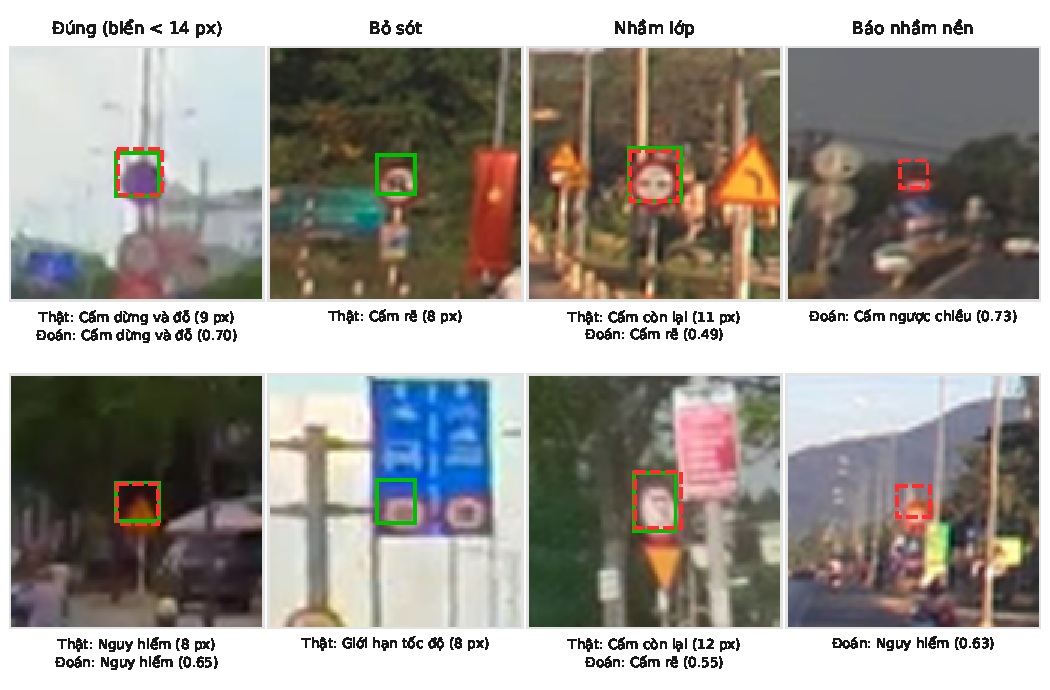
\includegraphics[width=0.92\textwidth]{figures/vi_du_du_doan.pdf}
\caption{Ví dụ dự đoán của YOLOv8s 1280 trên tập test (khung xanh liền: nhãn thật; khung đỏ đứt: dự đoán).
Cột 3, hàng dưới: biển có mũi tên rẽ bị gạch (\textit{Cấm rẽ}) nhưng bị gán nhãn \textit{Cấm còn lại}, nên dự đoán đúng của mô hình bị tính là nhầm lớp.
Cột 4: dự đoán không có nhãn thật tương ứng; hàng dưới trúng một biển thật không được gán nhãn.}
\label{fig:examples}
\end{figure*}

\subsection{Biển đứng cụm không bị bỏ sót nhiều hơn}
\label{sec:clusters}

43\% biển trong test đứng sát một biển khác (khe hở nhỏ hơn nửa cạnh của biển nhỏ hơn), thường là nhiều biển gắn trên cùng một cột.
Nếu chỉ nhìn số chung, biển trong cụm có vẻ bị bỏ sót nhiều hơn: recall 73,8\% so với 79,5\% với YOLOv8s 1280.
Nhưng biển trong cụm nhỏ hơn nhiều: 67,6\% dưới 16 pixel, so với 45,8\% ở biển đứng riêng.
Khi so trong từng nhóm kích thước, biển trong cụm được tìm thấy ngang bằng hoặc nhiều hơn (8--16 pixel: 86,0\% so với 77,7\%).
Vậy chênh lệch chung là do kích thước biển (biến gây nhiễu), không phải do NMS xóa nhầm biển đứng sát nhau. Ngưỡng NMS 0,65 theo từng lớp là đủ an toàn.

\subsection{Thí nghiệm: rò rỉ dữ liệu khi chia ngẫu nhiên}
\label{sec:leakage}

Để đo tác động của cách chia tập, nhóm lấy tập train (2.933 ảnh, 28 tuyến đường) chia lại thành train$'$/val$'$ (1.994/939 ảnh) theo hai cách: ngẫu nhiên theo ảnh, và theo tuyến đường.
Hai mô hình YOLOv8n (imgsz 1280, 50 epoch, cùng seed) được huấn luyện giống hệt nhau, chỉ khác cách chia.
Cả hai được chấm trên val$'$ của chính nó, và trên tập val gốc gồm 5 tuyến đường cả hai chưa từng thấy (Bảng~\ref{tab:leakage}). Tập test không được dùng trong thí nghiệm này.

\begin{table}[t]
\centering
\small
\begin{tabular}{lccc}
\toprule
Cách chia & val$'$ & Đường mới & Chênh \\
\midrule
Ngẫu nhiên    & \textbf{78,5} & \textbf{72,8} & $+5{,}7$ \\
Theo đường    & 62,9 & 69,9 & $-7{,}0$ \\
\bottomrule
\end{tabular}
\caption{mAP@0.5 (\%) của thí nghiệm rò rỉ. Với cách chia ngẫu nhiên, 88\% ảnh val$'$ có khung hình liền kề nằm trong train$'$.}
\label{tab:leakage}
\end{table}

Trên val$'$, mô hình chia ngẫu nhiên hơn mô hình chia theo đường 15,6 điểm. Trên cùng các tuyến đường mới, nó chỉ hơn 2,9 điểm.
Vậy phần lớn khoảng cách trên val$'$ là ảo: 88\% ảnh val$'$ có một khung hình gần như giống hệt trong train$'$.
Nếu tin vào val$'$ chia ngẫu nhiên, ta đánh giá khả năng trên đường mới cao hơn thực tế 5,7 điểm.
Phần hơn 2,9 điểm còn lại có thể vì mô hình chia ngẫu nhiên được thấy cả 28 tuyến đường, còn mô hình kia chỉ thấy 23.
Thí nghiệm cũng cho thấy hai bộ 5 tuyến đường có thể chênh nhau tới 7 điểm (62,9 so với 69,9). Điều này giúp giải thích vì sao kết quả trên val và test của nhóm lệch nhau 5--6 điểm.

\subsection{Thí nghiệm: xử lý mất cân bằng lớp}
\label{sec:imbalance}

Mục~\ref{sec:confusion} cho thấy các lớp ít mẫu (\textit{Cấm rẽ}, \textit{Giới hạn tốc độ}) cũng là các lớp hay bị nhầm. Nhóm thử hai cách cân bằng lớp trên cấu hình YOLOv8s 1280, mỗi cách chỉ thay đổi đúng một yếu tố:
\begin{itemize}
\item \textbf{Repeat Factor Sampling} (RFS) \citep{gupta2019lvis}: lặp lại các ảnh chứa lớp hiếm với hệ số $r_c = \max(1, \sqrt{t/f_c})$, trong đó $f_c$ là tỉ lệ ảnh có lớp $c$ và $t = 0{,}3$. Cách này giảm tỉ lệ số box lớp nhiều nhất / ít nhất từ 4,4 xuống 2,9.
\item \textbf{Trọng số lớp} trong loss phân loại, tỉ lệ với $(1/n_c)^{0{,}5}$, trong đó $n_c$ là số box của lớp $c$ (tham số \texttt{cls\_pw} của Ultralytics).
\end{itemize}

\begin{table}[t]
\centering
\small
\begin{tabular}{lccc}
\toprule
& Gốc & RFS & Trọng số lớp \\
\midrule
mAP@0.5          & \textbf{82,2} & 81,0 & 81,1 \\
AP50 Cấm rẽ          & \textbf{75,0} & 71,4 & 74,9 \\
AP50 Giới hạn tốc độ & \textbf{77,7} & 73,1 & 71,6$^{*}$ \\
AP50 Hiệu lệnh       & 78,6 & \textbf{80,7} & 78,7 \\
Nhầm trong nhóm tròn đỏ & \textbf{47} & 56 & 50 \\
\bottomrule
\end{tabular}
\caption{Thí nghiệm mất cân bằng lớp trên val (\%). Dòng cuối là số biển bị nhầm giữa ba lớp tròn viền đỏ. $^{*}$: chênh lệch so với gốc có ý nghĩa thống kê (bootstrap, khoảng tin cậy 95\% là $[-10{,}2; -1{,}6]$). Mọi chênh lệch khác đều nằm trong khoảng dao động.}
\label{tab:imbalance}
\end{table}

Cả hai cách đều \emph{không} cải thiện các lớp hiếm (Bảng~\ref{tab:imbalance}). Có bốn nguyên nhân:
\begin{enumerate}
\item \textbf{Lỗi chỉ bị chuyển chỗ, không mất đi.} Tổng số lần nhầm trong nhóm tròn đỏ không giảm (47 tăng lên 56 và 50).
  Với trọng số lớp, \textit{Cấm rẽ} được nhận đúng thêm 3 biển, nhưng số dự đoán \textit{Cấm rẽ} sai tăng từ 9 lên 17. \textit{Giới hạn tốc độ} bị kéo sang \textit{Cấm rẽ} nhiều hơn, nên AP của nó giảm 6,1 điểm.
  Trọng số chỉ dịch ranh giới quyết định giữa các lớp trông giống nhau, chứ không giúp phân biệt chúng tốt hơn.
\item \textbf{Lặp ảnh thì lặp luôn lớp gây nhầm.} 49\% ảnh có \textit{Giới hạn tốc độ} cũng có \textit{Cấm còn lại}, trong khi tỉ lệ chung chỉ 25\%. Vì vậy RFS lặp chính lớp mà \textit{Giới hạn tốc độ} hay bị nhầm sang.
\item \textbf{Nhầm lớp không phải lỗi chính.} Chỉ 3,2\% biển bị nhầm lớp, trong khi 16,7\% bị bỏ sót (Mục~\ref{sec:small}). Cân bằng lớp không làm recall biển nhỏ tăng.
\item \textbf{Mức mất cân bằng vừa phải} (4,4 lần). RFS được thiết kế cho dữ liệu đuôi dài, nơi lớp hiếm ít hơn hàng trăm lần.
\end{enumerate}
Không thấy dấu hiệu học thuộc do lặp ảnh: loss phân loại trên val vẫn giảm tới epoch cuối.
Với nhầm lẫn giữa các lớp tròn viền đỏ, cách hợp lý hơn là cho mô hình nhìn rõ phần giữa biển (độ phân giải cao hơn, hoặc phân loại lại vùng cắt quanh biển) và sửa nhãn sai (Mục~\ref{sec:confusion}).

\subsection{Hạn chế}
\label{sec:limitations}

\begin{itemize}
\item \textbf{Nhãn còn nhiễu.} Box trùng đã được gộp, nhưng nhãn sai lớp và biển thiếu nhãn vẫn còn (Mục~\ref{sec:confusion} và \ref{sec:missing-labels}). Điểm trên test vì vậy là cận dưới của khả năng thật.
\item \textbf{Ít tuyến đường.} Val và test mỗi tập chỉ có 5 tuyến đường. Kết quả có thể lệch vài điểm tùy tuyến đường nào rơi vào tập nào (Mục~\ref{sec:leakage}).
\item \textbf{Mỗi cấu hình chỉ huấn luyện một lần.} Khoảng tin cậy bootstrap chỉ tính dao động do chọn ảnh, chưa tính dao động giữa các lần huấn luyện.
\item \textbf{AP\textsubscript{L} không đáng tin.} Val chỉ có 23 biển lớn và test có 34, nên nhóm không so sánh AP\textsubscript{L}.
\item \textbf{Ngưỡng xuất dự đoán của Faster R-CNN trên val} là 0,05 thay vì 0,001, nên mAP trên val của Faster R-CNN có thể thấp hơn thực tế một chút. Trên test thì không có vấn đề này.
\end{itemize}

% Cần: booktabs, graphicx; hình trong figures/ (tạo bằng docs/report/make_figures.py)
% Số liệu: reports/errors/*_test, experiments/leakage, experiments/imbalance
% ------------------------------------------------

\section{Phân tích}
\label{sec:analysis}

Mục này dùng các mô hình cuối trên tập test (1.748 biển) để tách lỗi thành ba loại, theo cách ghép dự đoán với nhãn ở IoU $\geq 0{,}5$:
\begin{itemize}
\item \emph{bỏ sót}: không có dự đoán nào trùng biển;
\item \emph{nhầm lớp}: dự đoán trùng biển nhưng sai lớp;
\item \emph{báo nhầm nền}: dự đoán không trùng biển nào.
\end{itemize}
Ngưỡng độ tin cậy của mỗi mô hình được chọn sao cho F1 cao nhất, vì thang điểm tin cậy của YOLO và Faster R-CNN khác nhau. Phân tích trên tập val cho cùng các kết luận.

\subsection{Lỗi chính là bỏ sót biển nhỏ}
\label{sec:small}

Với YOLOv8s 1280, 77,1\% biển được tìm đúng, 21,1\% bị bỏ sót, và chỉ 1,9\% bị nhận sai lớp.
Trong 368 biển bị bỏ sót, 337 biển (92\%) nhỏ hơn 16 pixel. Hai mô hình còn lại cũng như vậy: 91\% với cắt ô + SAHI và 87\% với Faster R-CNN.
Hình~\ref{fig:recall-size} cho thấy với YOLO, recall gần như bão hòa ($> 92\%$) ở biển từ 16 pixel trở lên. Recall giảm ở biển 8--16 pixel, và ở biển dưới 8 pixel chỉ còn 21--39\% với cả ba mô hình.
Ở imgsz 1280, một biển 8 pixel trên ảnh gốc chỉ còn khoảng 6 pixel, nhỏ hơn một ô của bản đồ đặc trưng mịn nhất của YOLOv8 (stride 8). Cắt ô giữ nguyên độ phân giải gốc, nên tăng recall ở nhóm này từ 33,0\% lên 38,7\%.

Faster R-CNN kém YOLO ở mọi nhóm kích thước, kể cả nhóm $\geq 32$ pixel (93,6\% so với 96,4\%). Ảnh đưa vào Faster R-CNN còn lớn hơn (cạnh dài 1800 pixel), nên khoảng cách này không đến từ độ phân giải. Nhiều khả năng nó đến từ thiết lập huấn luyện: 30 epoch, augmentation đơn giản, so với 50 epoch có mosaic của YOLO. Faster R-CNN cũng báo nhầm nền nhiều hơn (156 so với 97 box).

\begin{figure}[t]
\centering
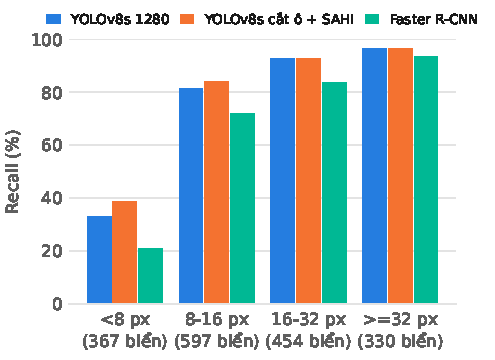
\includegraphics[width=\columnwidth]{figures/recall_theo_kich_thuoc.pdf}
\caption{Recall theo kích thước biển ($\sqrt{wh}$ trên ảnh gốc), tập test. Số dưới trục là số biển trong mỗi nhóm.}
\label{fig:recall-size}
\end{figure}

\subsection{Nhầm lớp tập trung ở ba lớp biển tròn viền đỏ}
\label{sec:confusion}

Ở YOLOv8s 1280, 30 trong 33 lần nhầm lớp (91\%) xảy ra giữa \textit{Cấm rẽ}, \textit{Giới hạn tốc độ} và \textit{Cấm còn lại}. Tỉ lệ bị gán sai lớp của ba lớp này lần lượt là 9,9\%, 11,4\% và 8,5\%, trong khi bốn lớp còn lại không quá 0,4\%.
Ba lớp này có cùng hình tròn, nền trắng, viền đỏ, chỉ khác hình vẽ ở giữa. Với biển 10 pixel, phần ở giữa chỉ còn vài pixel.
\textit{Cấm ngược chiều} là trường hợp ngược lại: lớp này có tới 90,5\% box nhỏ nhưng vẫn đạt AP50 84,7 trên test, vì nền đỏ đặc với vạch trắng ngang không giống lớp nào khác.
Vì vậy, độ khó của một lớp phụ thuộc vào việc nó có giống lớp khác không, hơn là vào kích thước biển.
Faster R-CNN nhầm nặng hơn hẳn: 28,4\% biển \textit{Cấm rẽ} bị gán sai lớp, chủ yếu thành \textit{Cấm còn lại}.

Nhóm xem lại bằng mắt cả 33 trường hợp nhầm lớp của YOLOv8s 1280:
\begin{itemize}
\item Ít nhất 7 trường hợp là \emph{nhãn sai, mô hình đúng}: biển ``50'' và ``80'' bị ghi \textit{Cấm còn lại}, biển hạn chế tải trọng ``10T'' bị ghi \textit{Giới hạn tốc độ}, biển tam giác cảnh báo bị ghi \textit{Hiệu lệnh}.
\item 4 trường hợp là lỗi rõ ràng của mô hình, ví dụ biển cấm rẽ rõ nét bị đoán thành \textit{Giới hạn tốc độ}.
\item Khoảng 19 trường hợp còn lại quá nhỏ hoặc quá mờ để người xem phân xử.
\end{itemize}

\subsection{Một phần ``báo nhầm nền'' là biển thiếu nhãn}
\label{sec:missing-labels}

Nhóm cũng xem lại 28 dự đoán bị tính là báo nhầm nền có độ tin cậy $\geq 0{,}6$, tức là các dự đoán không chồng lên box thật nào.
Ít nhất 15 trường hợp trúng một biển báo rõ ràng thuộc 7 lớp nhưng không được gán nhãn. Ví dụ: biển cấm đỗ và biển cấm rẽ trên cùng một cột, biển cảnh báo tam giác, biển ``10'' (Hình~\ref{fig:examples}, cột cuối).
Khoảng 5 trường hợp khác có thể cũng là biển. Chỉ khoảng 8 trường hợp là nền thật, chủ yếu là các mảng tối mờ.
Như vậy, nhãn test vừa thiếu biển vừa có nhãn sai lớp, và cả hai đều làm điểm của mô hình thấp hơn khả năng thật. Mức chênh này chưa được định lượng.

\begin{figure*}[t]
\centering
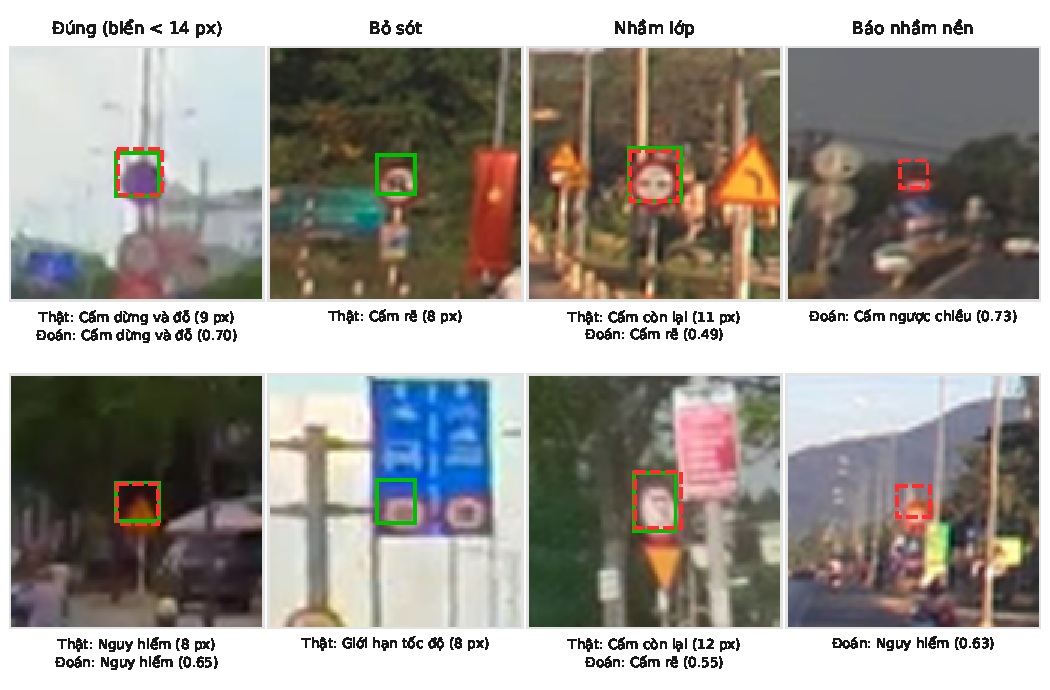
\includegraphics[width=0.92\textwidth]{figures/vi_du_du_doan.pdf}
\caption{Ví dụ dự đoán của YOLOv8s 1280 trên tập test (khung xanh liền: nhãn thật; khung đỏ đứt: dự đoán).
Cột 3, hàng dưới: biển có mũi tên rẽ bị gạch (\textit{Cấm rẽ}) nhưng bị gán nhãn \textit{Cấm còn lại}, nên dự đoán đúng của mô hình bị tính là nhầm lớp.
Cột 4: dự đoán không có nhãn thật tương ứng; hàng dưới trúng một biển thật không được gán nhãn.}
\label{fig:examples}
\end{figure*}

\subsection{Biển đứng cụm không bị bỏ sót nhiều hơn}
\label{sec:clusters}

43\% biển trong test đứng sát một biển khác (khe hở nhỏ hơn nửa cạnh của biển nhỏ hơn), thường là nhiều biển gắn trên cùng một cột.
Nếu chỉ nhìn số chung, biển trong cụm có vẻ bị bỏ sót nhiều hơn: recall 73,8\% so với 79,5\% với YOLOv8s 1280.
Nhưng biển trong cụm nhỏ hơn nhiều: 67,6\% dưới 16 pixel, so với 45,8\% ở biển đứng riêng.
Khi so trong từng nhóm kích thước, biển trong cụm được tìm thấy ngang bằng hoặc nhiều hơn (8--16 pixel: 86,0\% so với 77,7\%).
Vậy chênh lệch chung là do kích thước biển (biến gây nhiễu), không phải do NMS xóa nhầm biển đứng sát nhau. Ngưỡng NMS 0,65 theo từng lớp là đủ an toàn.

\subsection{Thí nghiệm: rò rỉ dữ liệu khi chia ngẫu nhiên}
\label{sec:leakage}

Để đo tác động của cách chia tập, nhóm lấy tập train (2.933 ảnh, 28 tuyến đường) chia lại thành train$'$/val$'$ (1.994/939 ảnh) theo hai cách: ngẫu nhiên theo ảnh, và theo tuyến đường.
Hai mô hình YOLOv8n (imgsz 1280, 50 epoch, cùng seed) được huấn luyện giống hệt nhau, chỉ khác cách chia.
Cả hai được chấm trên val$'$ của chính nó, và trên tập val gốc gồm 5 tuyến đường cả hai chưa từng thấy (Bảng~\ref{tab:leakage}). Tập test không được dùng trong thí nghiệm này.

\begin{table}[t]
\centering
\small
\begin{tabular}{lccc}
\toprule
Cách chia & val$'$ & Đường mới & Chênh \\
\midrule
Ngẫu nhiên    & \textbf{78,5} & \textbf{72,8} & $+5{,}7$ \\
Theo đường    & 62,9 & 69,9 & $-7{,}0$ \\
\bottomrule
\end{tabular}
\caption{mAP@0.5 (\%) của thí nghiệm rò rỉ. Với cách chia ngẫu nhiên, 88\% ảnh val$'$ có khung hình liền kề nằm trong train$'$.}
\label{tab:leakage}
\end{table}

Trên val$'$, mô hình chia ngẫu nhiên hơn mô hình chia theo đường 15,6 điểm. Trên cùng các tuyến đường mới, nó chỉ hơn 2,9 điểm.
Vậy phần lớn khoảng cách trên val$'$ là ảo: 88\% ảnh val$'$ có một khung hình gần như giống hệt trong train$'$.
Nếu tin vào val$'$ chia ngẫu nhiên, ta đánh giá khả năng trên đường mới cao hơn thực tế 5,7 điểm.
Phần hơn 2,9 điểm còn lại có thể vì mô hình chia ngẫu nhiên được thấy cả 28 tuyến đường, còn mô hình kia chỉ thấy 23.
Thí nghiệm cũng cho thấy hai bộ 5 tuyến đường có thể chênh nhau tới 7 điểm (62,9 so với 69,9). Điều này giúp giải thích vì sao kết quả trên val và test của nhóm lệch nhau 5--6 điểm.

\subsection{Thí nghiệm: xử lý mất cân bằng lớp}
\label{sec:imbalance}

Mục~\ref{sec:confusion} cho thấy các lớp ít mẫu (\textit{Cấm rẽ}, \textit{Giới hạn tốc độ}) cũng là các lớp hay bị nhầm. Nhóm thử hai cách cân bằng lớp trên cấu hình YOLOv8s 1280, mỗi cách chỉ thay đổi đúng một yếu tố:
\begin{itemize}
\item \textbf{Repeat Factor Sampling} (RFS) \citep{gupta2019lvis}: lặp lại các ảnh chứa lớp hiếm với hệ số $r_c = \max(1, \sqrt{t/f_c})$, trong đó $f_c$ là tỉ lệ ảnh có lớp $c$ và $t = 0{,}3$. Cách này giảm tỉ lệ số box lớp nhiều nhất / ít nhất từ 4,4 xuống 2,9.
\item \textbf{Trọng số lớp} trong loss phân loại, tỉ lệ với $(1/n_c)^{0{,}5}$, trong đó $n_c$ là số box của lớp $c$ (tham số \texttt{cls\_pw} của Ultralytics).
\end{itemize}

\begin{table}[t]
\centering
\small
\begin{tabular}{lccc}
\toprule
& Gốc & RFS & Trọng số lớp \\
\midrule
mAP@0.5          & \textbf{82,2} & 81,0 & 81,1 \\
AP50 Cấm rẽ          & \textbf{75,0} & 71,4 & 74,9 \\
AP50 Giới hạn tốc độ & \textbf{77,7} & 73,1 & 71,6$^{*}$ \\
AP50 Hiệu lệnh       & 78,6 & \textbf{80,7} & 78,7 \\
Nhầm trong nhóm tròn đỏ & \textbf{47} & 56 & 50 \\
\bottomrule
\end{tabular}
\caption{Thí nghiệm mất cân bằng lớp trên val (\%). Dòng cuối là số biển bị nhầm giữa ba lớp tròn viền đỏ. $^{*}$: chênh lệch so với gốc có ý nghĩa thống kê (bootstrap, khoảng tin cậy 95\% là $[-10{,}2; -1{,}6]$). Mọi chênh lệch khác đều nằm trong khoảng dao động.}
\label{tab:imbalance}
\end{table}

Cả hai cách đều \emph{không} cải thiện các lớp hiếm (Bảng~\ref{tab:imbalance}). Có bốn nguyên nhân:
\begin{enumerate}
\item \textbf{Lỗi chỉ bị chuyển chỗ, không mất đi.} Tổng số lần nhầm trong nhóm tròn đỏ không giảm (47 tăng lên 56 và 50).
  Với trọng số lớp, \textit{Cấm rẽ} được nhận đúng thêm 3 biển, nhưng số dự đoán \textit{Cấm rẽ} sai tăng từ 9 lên 17. \textit{Giới hạn tốc độ} bị kéo sang \textit{Cấm rẽ} nhiều hơn, nên AP của nó giảm 6,1 điểm.
  Trọng số chỉ dịch ranh giới quyết định giữa các lớp trông giống nhau, chứ không giúp phân biệt chúng tốt hơn.
\item \textbf{Lặp ảnh thì lặp luôn lớp gây nhầm.} 49\% ảnh có \textit{Giới hạn tốc độ} cũng có \textit{Cấm còn lại}, trong khi tỉ lệ chung chỉ 25\%. Vì vậy RFS lặp chính lớp mà \textit{Giới hạn tốc độ} hay bị nhầm sang.
\item \textbf{Nhầm lớp không phải lỗi chính.} Chỉ 3,2\% biển bị nhầm lớp, trong khi 16,7\% bị bỏ sót (Mục~\ref{sec:small}). Cân bằng lớp không làm recall biển nhỏ tăng.
\item \textbf{Mức mất cân bằng vừa phải} (4,4 lần). RFS được thiết kế cho dữ liệu đuôi dài, nơi lớp hiếm ít hơn hàng trăm lần.
\end{enumerate}
Không thấy dấu hiệu học thuộc do lặp ảnh: loss phân loại trên val vẫn giảm tới epoch cuối.
Với nhầm lẫn giữa các lớp tròn viền đỏ, cách hợp lý hơn là cho mô hình nhìn rõ phần giữa biển (độ phân giải cao hơn, hoặc phân loại lại vùng cắt quanh biển) và sửa nhãn sai (Mục~\ref{sec:confusion}).

\subsection{Hạn chế}
\label{sec:limitations}

\begin{itemize}
\item \textbf{Nhãn còn nhiễu.} Box trùng đã được gộp, nhưng nhãn sai lớp và biển thiếu nhãn vẫn còn (Mục~\ref{sec:confusion} và \ref{sec:missing-labels}). Điểm trên test vì vậy là cận dưới của khả năng thật.
\item \textbf{Ít tuyến đường.} Val và test mỗi tập chỉ có 5 tuyến đường. Kết quả có thể lệch vài điểm tùy tuyến đường nào rơi vào tập nào (Mục~\ref{sec:leakage}).
\item \textbf{Mỗi cấu hình chỉ huấn luyện một lần.} Khoảng tin cậy bootstrap chỉ tính dao động do chọn ảnh, chưa tính dao động giữa các lần huấn luyện.
\item \textbf{AP\textsubscript{L} không đáng tin.} Val chỉ có 23 biển lớn và test có 34, nên nhóm không so sánh AP\textsubscript{L}.
\item \textbf{Ngưỡng xuất dự đoán của Faster R-CNN trên val} là 0,05 thay vì 0,001, nên mAP trên val của Faster R-CNN có thể thấp hơn thực tế một chút. Trên test thì không có vấn đề này.
\end{itemize}
